% Please use the review version when submitting papers for review.
% The option below provides the final form of your paper

%\documentclass[review,article]{ij4uq}      %  review version
\documentclass[article]{ij4uq}              %  final version
% Use option "equation" for numbering equation as section

%\count0=115

% Added by author
\usepackage{graphicx}
\usepackage{caption}
\usepackage{subcaption}
\usepackage{stfloats}
\usepackage{fixltx2e}
\usepackage{placeins}

% \newcommand{\thesubfigure} [\alph{subfigure}]


%\fancypagestyle{plain}{%
%  \fancyhf{}
%  \fancyhead[R]{\small {\it DynaSearch User's Manual}, 1(1):xxx--xxx, \myyear\today}
%  \fancyfoot[R]{\vspace*{10pt}\small\bf\thepage }
%  \fancyfoot[L]{\fottitle}
%  }


\begin{document}

\volume{Volume 1, Number 1, \myyear\today}
\title{DynaSearch User's Manual}
\titlehead{DynaSearch User's Manual}
\authorhead{Cox, Malloy, House, \& Lindell}

% For authors with the same post address, uncomment the following
% 7 lines

\corrauthor[1]{Jonathan Cox}
\author[1]{Chris Malloy}
\author[1]{Jordan Gestring}
\author[1]{Donald House}
\author[2]{Michael Lindell}
\corremail{jlcox@g.clemson.edu}
\corrurl{http://www.clemson.edu/ces/savage/}
\address[1]{ School of Computing, 100 McAdams Hall, Clemson University, Clemson, SC 29634-0974, USA}
\address[2]{Hazard Reduction \& Recovery Center, College of Architecture, Texas A\&M University, College Station, TX 77843-3137, USA}

% End commands for all authors with the same address

% For at least 2 authors with different addresses, use instead the following commands

%\author[1]{Xiang Ma}
%\email{xm25@cornell.edu}
%\author[2]{James Taylor}
%\email{taylor@cornell.edu}
%\corrauthor[2]{Nicholas Zabaras}
%\corremail{zabaras@cornell.edu}
%\corrurl{http://mpdc.mae.cornell.edu/}
%\address[1]{Materials Process Design and Control Laboratory, Sibley School of Mechanical and Aerospace
%Engineering, 101 Frank H.T. Rhodes Hall, Cornell University, Ithaca, NY 14853-3801, USA}
%\address[2]{Another Address Here,   Cornell University, Ithaca, NY 14853-3801, USA}

% End information for at least 2 authors with different addresses


\dataO{\mydate\today}
%\dataO{}
\dataF{\mydate\today}
%\dataF{}

\abstract{
}

% Up to seven key words are required. Please provide a list consulting
% the keywords given in the document IJ4UQ-KeyWords.pdf if different
% key words as needed.

\keywords{Experiment Design}


\maketitle




\section{Introduction}

DynaSearch is a web based system that allows the end user to create and run a variety of user studies.  The basic toolset supports the construction of studies designed to test how users collect and process information by recording the order and duration of mouse clicks on a set of pre-designed page elements, such as text boxes.  In addition, DynaSearch supports more complex user studies by allowing end users to write and embedd their own custom experiements through the use of Java Applets, HTLM5, WebGL, Processing, and D3.  The rest of this document will explain these tools in greater detail, but in order to provide you with an overall picture of the product, a simple example of what can be created is detailed below.

\subsection{A Short Example}

\subsubsection{The Login Screen}

\begin{figure}[h!]
 \centering
 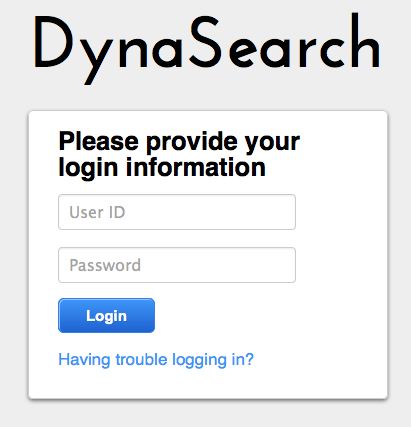
\includegraphics[width=2.0in]{figures/ds_login.png}
 \caption{Users will start an experiment by logging into the DynaSearch system through the login screen.}
 \label{fig:login}
\end{figure}
\FloatBarrier

All users should be provided with a user name and password so that they may login to the system. User accounts can be created and edited within the Manage Participants window. The login screen is displayed in \ref{fig:login}.

\subsubsection{The Size Registration Screen}

\begin{figure}[h!]
 \centering
 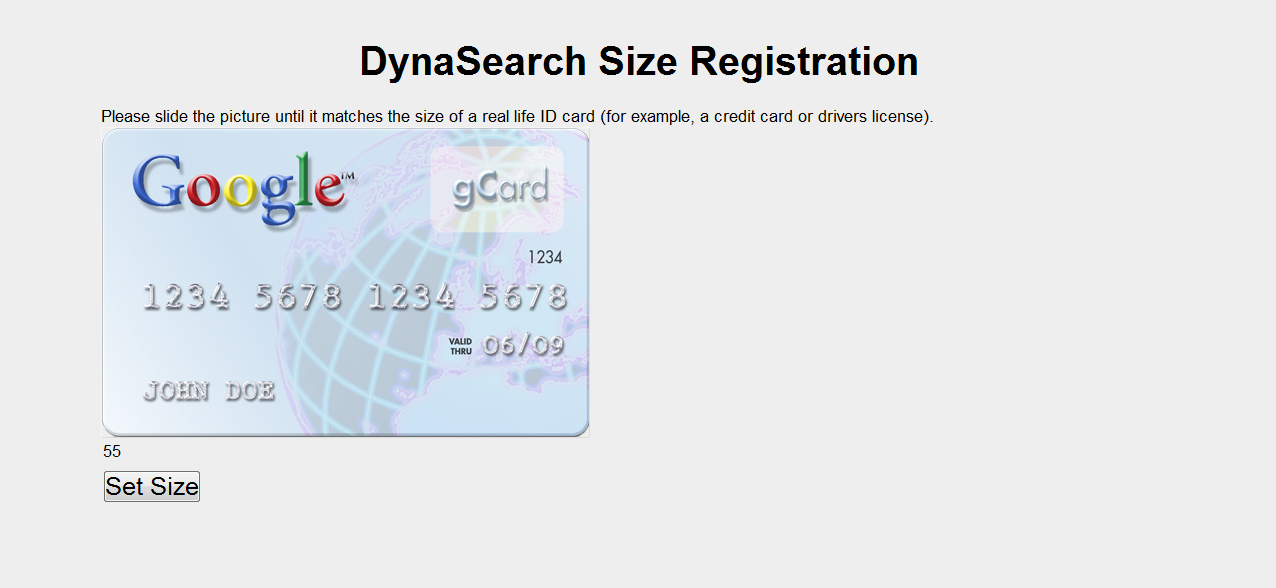
\includegraphics[width=4.0in]{figures/size_reg.png}
 \caption{Users must first register the size of their screen.}
 \label{fig:sizereg}
\end{figure}
\FloatBarrier


In order to ensure that all users see screen elements of the exact same size, regardless of screen size and resolution, a size registration may be required by an experiement. This is done by holding a physical credit card up to the screen and sliding the edges of the Google credit card image until it is the same size as the physical card. This screen is shown in Fig. \ref{fig:sizereg}.

\subsubsection{The Instruction Screen}

\begin{figure}[h!]
 \centering
 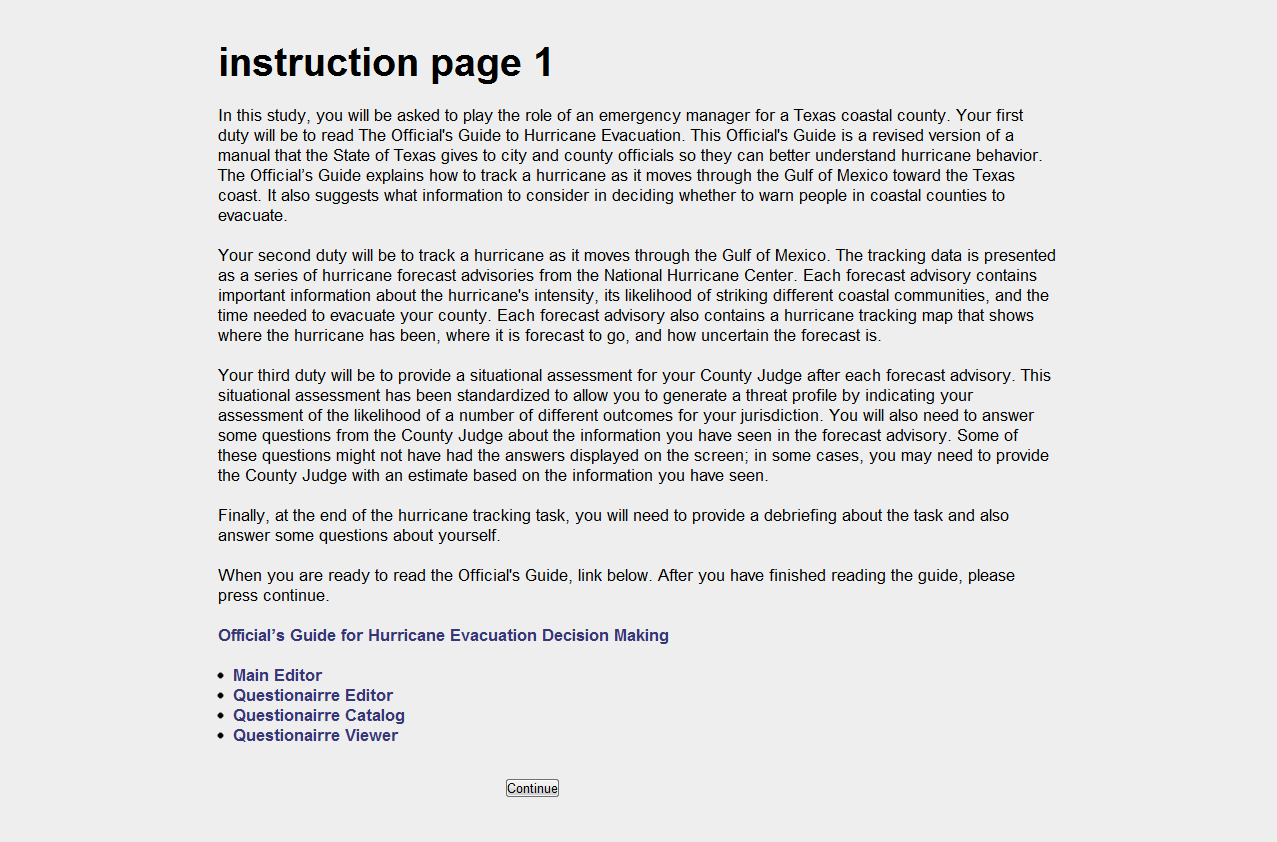
\includegraphics[width=4.0in]{figures/instruction_page.png}
 \caption{The instruction screen displays information for the users.}
 \label{fig:inst}
\end{figure}
\FloatBarrier

Users can be supplied with supplemental information using the instruction screen. A sample instruction screen is displayed in Fig. \ref{fig:inst}.  Instruction pages can be as simple as plain text.  However, they are read as HTML files and can be expanded to include any valid HTML tags as well as script components.

\begin{figure}[h!]
 \centering
 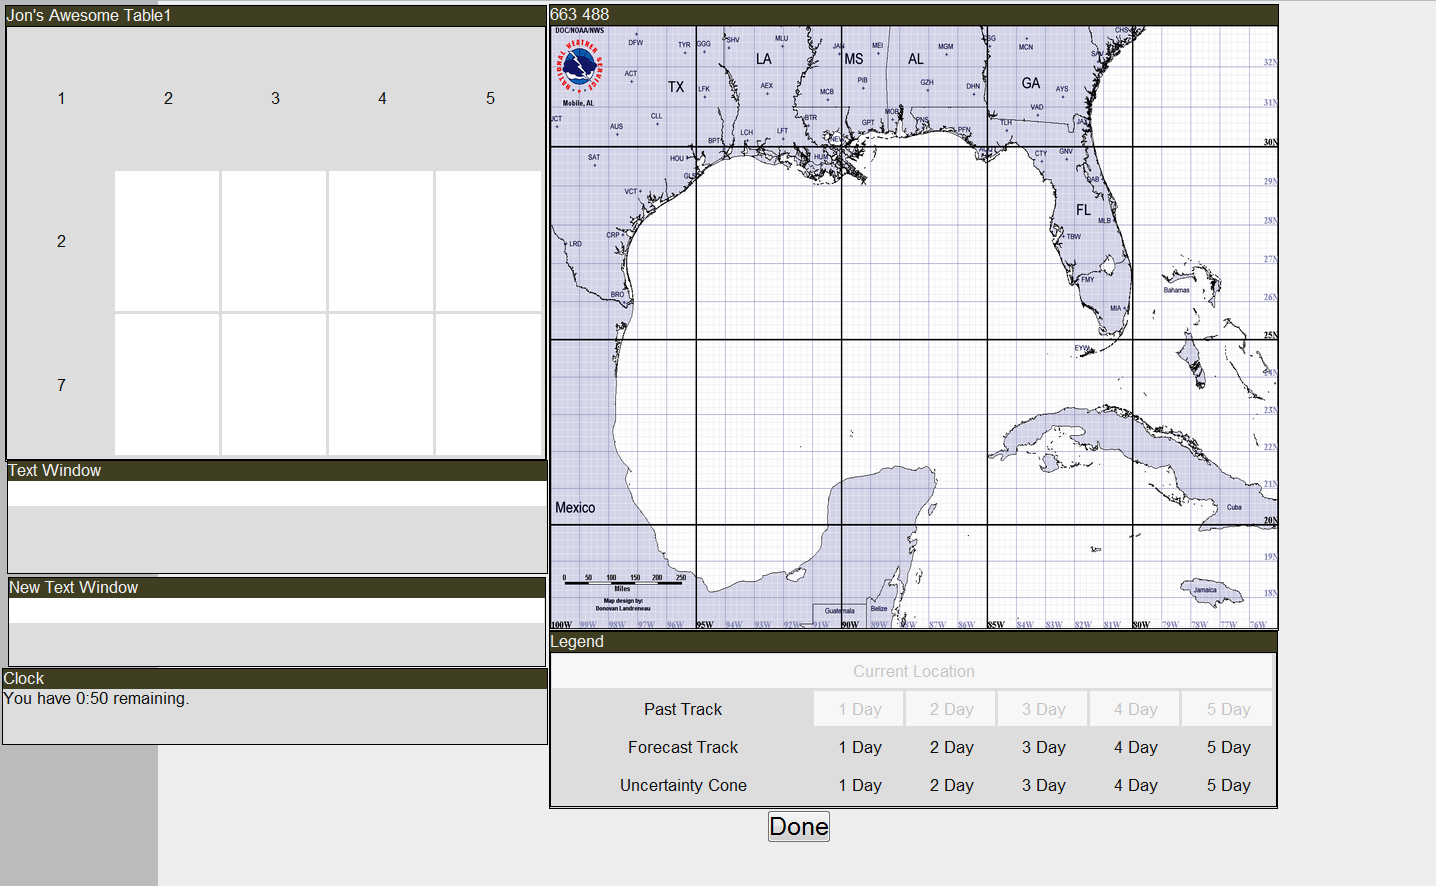
\includegraphics[width=4.0in]{figures/training_page.png}
 \caption{The training screen records information based on user clicks.}
 \label{fig:train}
\end{figure}
\FloatBarrier

\subsubsection{The Training Screen}

The training screen records the order and duration of participant clicks. The participant clicks on the screen in order to uncover certain pieces of information, whether it is a cell of a table or information drawn over an image. A sample training screen is displayed in Fig. \ref{fig:train}.  Training screens can include a timer which will force participants to move to the next portion of the experiment after a defined period of time.  Training screens also support embedded Java applets, HTML 5 pages that utilize WebGL, Processing, and D3.  This will be explained in greater detail in the section of the manual that covers building training pages.

\subsubsection{The Survey Screen}

\begin{figure}[h!]
 \centering
 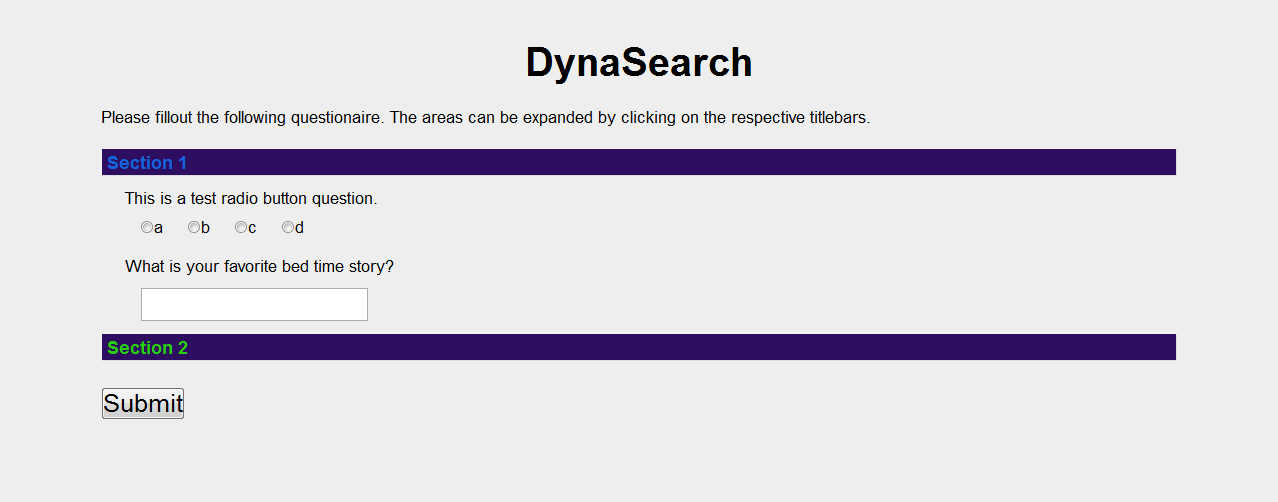
\includegraphics[width=5.0in]{figures/survey_page.png}
 \caption{The survey screen allows the users to answer specific questions.}
 \label{fig:survey}
\end{figure}
\FloatBarrier

The survey screen allows the participants to respond to specific questions designed by the end user. There are currently two question types available for use.  These are radio button questions and free response questions. A sample survey screen is displayed in Fig. \ref{fig:survey}.

%% \subsubsection{Complete Example}


%% \section{Introduction} %for journal use above \firstsection{..} instead

\section{Administrative Tools}

\subsection{A Quick Overview}
From this point forward, "you" will refer to the individual creating the experiments, and "user" refers to the research participants. 

The DynaSearch system allows for the creation of user studies that can be composed of three different types of pages. The first is the instruction page. Here, basic HTML is displayed that can be used to convey specific instructions to users or as a means of supplying them with supplemental information. The second is the training page. This page can be composed of text boxes, tables, and images that are all covered on the page's initial load.  In order for users to reveal the covered information and interact with any of these elements, they must click on it. The order and duration of these clicks is tracked by a database typically hosted on the web server. The training page can also house custom applets that offer a wider variety of interactions.  The last type of page is a questionnaire which gives users the opportunity to provide feedback.  Additionally, it can serve as a way to test the users on previously displayed information.

Accounts with administrator access are given access to the \textbf{Administrator's Page} where links to the different editors are listed. Instruction pages, training pages, and questionnaire pages can be created in any order. The experiment creation tool defines an experiement by linking pages together, and should not be used until all of the pages for a given experiment have been completed.

In addition to these editors, other pages have been provided to manage the assests used in an experiment, such as images or scripts, as well as to create users and access the data resulting from the experiments.   Assets used in the experienments can be managed through the \testbf{Asset Manager}.  The creation and editing of participant accounts can be completed through the \textbf{Participant Manager}, while their experimental results can be accessed through the \textbf{View Results} page.

The remainder of this section will explain the use and operation of these editors and pages. For more information regarding the database, please refer to Appendix A. For more information on the file system, please see Appendix B.

\subsubsection{Instruction Pages}
To create an instruction page, just create a text file that contains the information desired and upload it using the \textbf{Asset Manager}. Because this data will be inserted between the $<\texttt{body}>$ tags of the template instruction page, any additional HTML tags and scripting maybe used as desired. These files will automatically be available from the \textbf{Experiment Editor} editor page. 

\subsubsection{Training Pages}

\begin{figure}[h!]
 \centering
 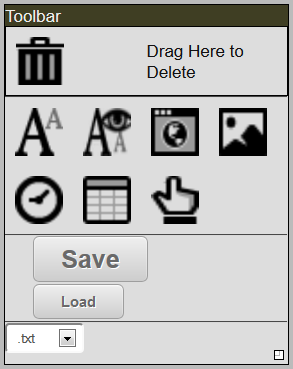
\includegraphics[width=2.0in]{figures/toolbar.png}
 \caption{The icons represent the trash bin, text window, visible text window, applet window, image window, clock, table window, interactive table window, and legend window respectively.}
 \label{fig:tool}
\end{figure}
\FloatBarrier

To access the training page, select the \textbf{Training Page Editor} link from the \textbf{Administrator's Page}. This will take you to a blank training editor page with the toolbar window located in the upper left window. With the exception of the trash can, each of the icons on the toolbar allow for the creation of a different window. The toolbar window is displayed in Figure \ref{fig:tool}. The toolbar window and any other created window can be moved by clicking and dragging on the title handle of the window.

\paragraph{The Trash Bin}
The Trash Bin allows you to delete unwanted windows. Simply click on the title bar of the window you wish to remove, and drag it over the trash can. When you release it, it will be deleted.

\paragraph{The Text Window}
The Text Window is used to display paragraphs or sections of text to the user. These will be hidden during a user study until the user clicks on the section containing the text. Both the title of the window and the text itself can be modified by clicking on the blue icon in the top right corner of the window. It can be resized by clicking and dragging on the white box in the bottom right corner of the window.

\paragraph{The Visible Text Window}
The Visible Text Window is similar to the Text Window, with the exception that the text will always be visible to users.  The contents will not be hidden during the course of a user study.

\begin{figure}[h!]
 \centering
 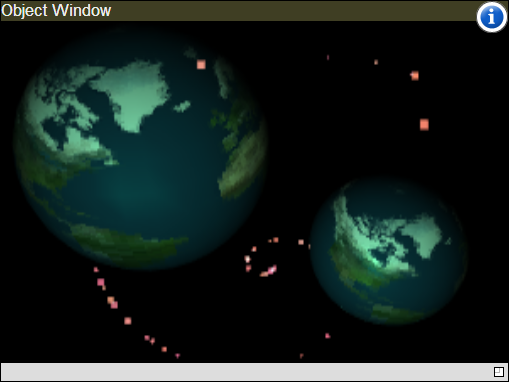
\includegraphics[width=4.0in]{figures/webgl.png}
 \caption{The Applet Window will let you embed various scripts and applets to extend the user study.}
 \label{fig:webgl}
\end{figure}
\FloatBarrier

\paragraph{The Applet Window}
The Applet Window lets you embed Java applets as well as HTML5 and JavaScript code that can include WebGL, Processing, or D3 scripts into the Training Page.  To assign an applet, HTML5, or JavaScript file to the Applet Window, click on the blue icon in the top right corner of the window and select the desired asset from the displayed dropdown menu.  Make sure that the asset has been uploaded using the \textbf{Asset Manager} before trying to load it into a applet object.  An example of the Applet Window can be seen in \ref{fig:webgl}.


\paragraph{The Image Window}
The Image Window allows you to display a static image.  The chosen image will always be displayed unless a Legend Window is associated with with it.  Please see the section covering the Legend Window for more information.  To select the image to be displayed, click on the blue icon in the top right corner of the window and and select the desired asset from the displayed dropdown menu.  Make sure that the asset has been uploaded using the \textbf{Asset Manager} before trying to load it into a image object.

\paragraph{The Clock Window}
The clock window determines how long a page will be available to a user. By clicking on the blue icon, you can specify the number of minutes that each user should receive. The default time is 20 minutes. If no clock window is created, then the window will be available to the user until they click on the Done button. Please note that the clock window will not actually be displayed while the experiment is being run.

\begin{figure}[h!]
 \centering
 \begin{subfigure}[b]{0.4\textwidth}
    \centering
    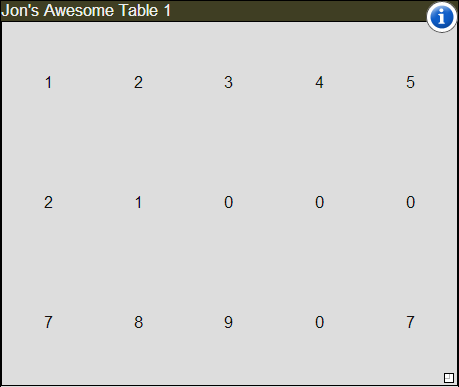
\includegraphics[width=2.0in]{figures/table_uncovered.png}
    \caption{In training page editor}
    \label{fig:tableUN}
 \end{subfigure}
 \begin{subfigure}[b]{0.4\textwidth}
    \centering
    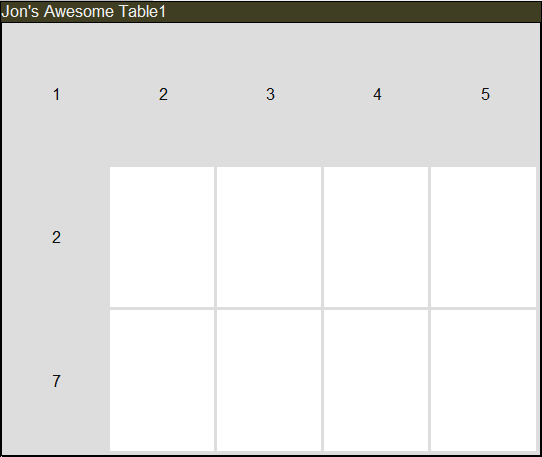
\includegraphics[width=2.0in]{figures/table_covered.png}
    \caption{Durring user study}
    \label{fig:tableCV}
 \end{subfigure}
 \caption{Table Window}
 \label{fig:tableWindow}
\end{figure}

%\begin{figure}[]
 %\centering
 %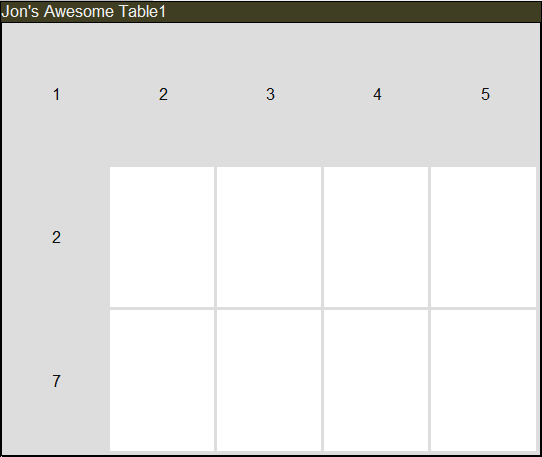
\includegraphics[width=2.0in]{figures/table_covered.png}
 %\caption{Table Window Covered}
 %\label{fig:table_cv}
%\end{figure}
\FloatBarrier

\paragraph{The Interactive Table Window}

The Interactive Table Window displays information in a table format, as demonstrated in \ref{fig:tableWindow}.  The first row and column will always be visible, while the other fields will be covered by a white box.  When clicked, the box will become transparent, allowing users to see the data values underneath.  Clicking on the blue icon will allow the user to change both the table name and the file in which the table data is stored. These text files are uploaded using the \textbf{Asset Manager}.  

When constructing the table files, columns are separated by commas, and the rows are separated by new lines. To resize the table, click and drag on the white box in the bottom right corner of the table window. You must resize the table manually in order to test that the information contained is displayed correctly.

In order to distinguish which table a user is clicking on from the entries in the database, the tables in an experiment should have unique table names.

\paragraph{The Table Window}

The Table Window behaves in the same manner as the Interactive Table Window with the exception that the data is visible at all times during the course of a user study.  Because of this, no click data is recorded for this type of table.

\paragraph{Loading A Training Page}
To load a previously saved training screen, pick the training file from the drop down menu that you wish to work with and hit the Load button. Note that to save any changes made to this training screen, you must hit the Save button before navigating away from the page.

\paragraph{Saving A Training Page}
The Save button will prompt you to enter a name to save the file as. The extension .txt will automatically be added to the name you supply, so it is not necessary to include that in the file name. For example, if you want the file name to be \texttt{test1.txt}, enter only \texttt{test1}.

\subsubsection {Questionnaire Editor}

\begin{figure}[h!]
 \centering
 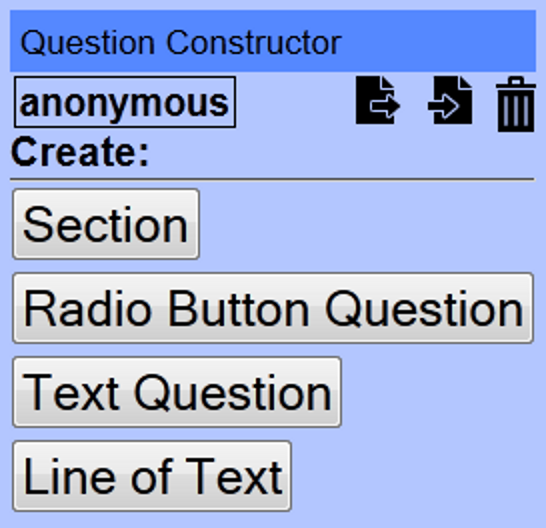
\includegraphics[width=5.0in]{figures/question_toolbar.png}
 \caption{Questionnaire Toolbar}
 \label{fig:questTool}
\end{figure}
\FloatBarrier

The Questionnaire Editor allows you to create a questionnaire that can be taken by users as they progress through an experiment. There are four basic building blocks that can be incorporated into a questionnaire, all of which are accessed through the interface displayed in Fig. \ref{fig:questTool}. In addition, the interface allows you to name, load, save, and clear the questionnaire currently being edited.

\begin{figure}[h!]
 \centering
 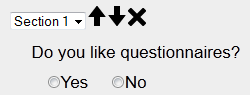
\includegraphics[width=2.5in]{figures/question_edit.png}
 \caption{Moving a Question}
 \label{fig:questEdit}
\end{figure}
\FloatBarrier

Questionnaires are built as a two tier hierarchy.  The top teir of this hierarchy can be composed of any of the building blocks, while the second tier can be composed of a set of radio button questions, text questions, and text that are nested under each section.  Sections are used to better organize questionnaires, and allow the users to control what questions are displayed at any time by expanding and collapsing the nested questions when a user clicks on the desired section's title bar.  

Questionnaire elements can be placed as desired throughout the questionnaire by using the controls located above each element as shown in Fig. \ref{fig:questEdit}.  To place an element within a specific section, select the desired section from the dropdown menu.  Please note that sections cannot be embedded within other sections.  To move a question or section up or down, use the up and down arrow buttons respectively.  Note that if an element is within a section, the arrow keys will only move it within that section. If the element is not located within a section, then it will navigate through the top tier.  To remove a question or section from the questionnaire completely, hit the \textbf{X} button.  \textbf{Be aware that if you delete a section that contains other elements, those other elements will also be deleted.}

When a questionnaire is completed by a user, their responses are saved and can be accessed and viewed through the \textbf{View Results} option from the \textbf{Administrator's Page}.

 Each of the building blocks and editing operations are described in greater detail below.

\paragraph{Section}
To create a section, hit the Section button from the Question Constructor toolbox and provide the desired name for the section at the given prompt.  When both fields have been completed, you can insert the section into the questionnaire by hitting the check mark button at the bottom of the prompt.  Sections allow you to segement a questionnaire into pieces.  When users are taking a questionnaire, these sections can be collapsed or expanded by clicking on the section's title bar.  Sections are for orgazational purposes only and do not affect the user output in any way.

At this time, sections are not able to contain other sections.  To remove or change the position of the radio button question, use the navigation controls located above the question as described above. \textbf{Be aware that if you delete a section that contains other elements, those other elements will also be deleted.}

\paragraph{Radio Button Question}
To create a radio button question, select the Radio Button Question button from the Question Constructor toolbox. DynaSearch will display a prompt for the question as well a text box for the first answer.  As soon as a value is typed in an answer box, a new box will be created underneath it.  In this way, the question can have as many choices as are needed.  The final empty box will not be displayed to the user when they take the questionnaire.  When all of the possible answers for the questions have been given, you can insert the question into the questionnaire by hitting the check mark button at the bottom of the prompt.

To remove or change the position of the radio button question after it has been inserted into the questionnaire, use the navigation controls located above the question as described above.  Note that DynaSearch will record the index value of the choice selected by the user, not the value you enter. 

\paragraph{Text Question}
To create a text question, select the Text Question button from the Question Constructor toolbox.  DynaSearch will display a prompt for the question as well as the max number of characters that should be allowed for the response.   For a free response question, use the number zero.  If the number of characters given is too large for the width of the screen, the text box created will have a tab on the lower right corner that can be dragged to increase its size.  When both fields have been completed, you can insert the question into the questionnaire by hitting the check mark button at the bottom of the prompt.

To remove or change the position of the text question after it has been inserted into the questionnaire, use the navigation controls located above the question as described above. 

\paragraph{Line of Text}
The Line of Text option allows you to provide users with additional instructions or information. After selecting this option and hitting the Next button, DynaSearch will prompt you to enter in the text that should be displayed. To add the information to the page, click the Next button again. To remove a line of text, simply click on the red minus symbol above the upper right corner of the element.

\paragraph{New}
The button labeled \textbf{New} clears the current questionnaire being edited and starts a new one.  The name of the questionnaire currently being edited is listed underneath the \textbf{New} button.

\paragraph{Save}
To save the questionnaire currently being edited, please click on the button labeled \textbf{Save}.  Please be aware that currently, DynaSearch will overwrite previous questionnaires of the same name without warning.

\paragraph{Save As}
To save the questionnaire currently being edited as a new questionnaire, please click on the button labeled \textbf{Save As}.  Please be aware that currently, DynaSearch will overwrite previous questionnaires of the same name without warning.

\paragraph{Delete}
To delete a questionnaire entirely, click on the button labeled \textbf{Delete}.  Please note that this will permanently remove a questionnaire from the list of available questionnaires to load.

\paragraph{Load}
To load a questionnaire, click the button labeled \textbf{Load}. DynaSearch will then display a prompt that allows you to select the questionnaire you wish to load from a dropdown box and selecting the green button labeled \textbf{Load}.

\paragraph{Append}
To load a previously written questionnaire into the questionnaire currently being edited, click on the button labeled \textbf{Append}.  This is useful if you have a segment of a questionnaire that needs to be inserted into many seperate questionnaires.  The segment can be saved individually, and then appeneded into each questionnaire seperately.  Please note that a questionnaire should not be appended to itself.  For any reason.  Yes, even that one.

\subsubsection{Experiment Editor}

\begin{figure}[h!]
 \centering
 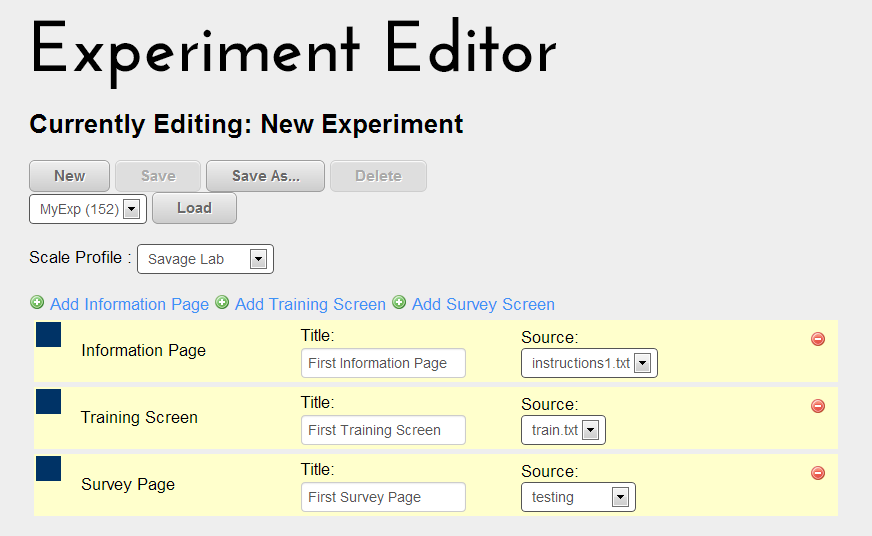
\includegraphics[width=5.0in]{figures/experiment_editor.png}
 \caption{Experiment Editor Interface}
 \label{fig:eeInterface}
\end{figure}
\FloatBarrier

The \textbf{Experiment Editor} allows you to combine any number of instruction pages, training pages, and questionnaires into a single experiment. The interface shown in \ref{fig:eeInterface} will allow you to select and assemble the various elements required. The experiment currently being edited is listed at the top following the line, "Currently Editing:".  When the page first loads, a new experiment entitled, "New Experiment" is created.

The remaining elements of the page are described in greater detail below.

\paragraph{New}
To start building a new experiment, click on the \textbf{New} button. Doing this will clear any work that has been done, so it is important to save previous work before continuing.

\paragraph{Save}
To save an experiment that you have been working on, click on the \textbf{Save} button.  How the experiements are saved is covered in greater detail in Apendix B.

\paragraph{Save As}
To save the experiment currently being edited as a different experiment, click on the \textbf{Save As} button.  You will be prompted to give a name for the experiement.  Please keep in mind that currently, DynaSearch does not check to determine if an experiment already exists with a name with you click on the \textbf{Save As} button.  This means that it is entirely possible to overwrite a prexisting experiment by entering it's name as the name to save the current experiment under.

\paragraph{Load Experiment}
To load a previously saved experiment, select the experiment that you wish to load from the drop down menu and then click on the \textbf{Load} button.  How experiments are saved is explained in greater detail in \textbf{Appendix B}.

\paragraph{Scale Profile}
Scale profiles adjust how the elements are scaled during an experiment.  If an experiement requires that users go through the size registration process to determine the scale needed, select \textem{Custom Scaling} from the scale profile menu dropdown.  Otherwise, select a specific profile from the list as needed by the experiement.  This will generaly want to match the profile used by the administrator when they were creating the experiment.

\paragraph{Add Information Page}

The \textbf{Add Information Page} link will allow you to insert a new information page into the current experiment. When this link is clicked, a new information page label is inserted into the current list of pages, as is shown in \ref{fig:infoInsert}.  To assign a title to the page, click on the box labed "Title" and insert the desired text.  The drop down box lists the current files that can be used as instruction pages.  The file used will be the one currently selected from the drop down menu.

To change the sequence of the pages, click and drag the blue box on the left hand side of a page label up or down to slide it into the desired location. To remove a page from your list of pages, select the red minus sign on the right hand side of its label.

\begin{figure}[htb]
 \centering
 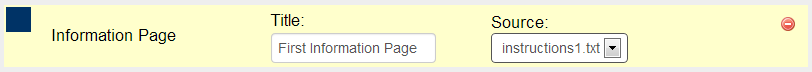
\includegraphics[width=5.0in]{figures/add_instruction.png}
 \caption{Information Page Inserted}
 \label{fig:infoInsert}
\end{figure}
\FloatBarrier

\paragraph{Add Training Page}

The \textbf{Add Training Page} link will allow you to insert a new training page into the current experiment. When this button is clicked, a new training page is inserted into the current list of pages, as is shown in \ref{fig:trainInsert}.  To assign a title to the page, click on the box labed "Title" and insert the desired text.  The drop down box lists the current training pages that are available.  The training page currently selected in the drop down box will be the one used during the experiement.

To change the sequence of a page, click and drag the blue box on the left hand side of the page label up or down to slide it into the desired location. To remove a page from your list of pages, select the red minus sign on the right hand side of its label.

\begin{figure}[h!]
 \centering
 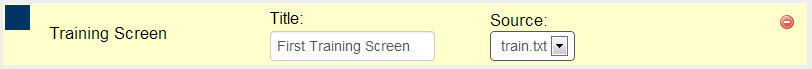
\includegraphics[width=5.0in]{figures/add_training.png}
 \caption{Training Page Inserted}
 \label{fig:trainInsert}
\end{figure}
\FloatBarrier

\paragraph{Add Survey Page}

The \textbf{Add Survey Page} link will allow you to insert a new questionnaire into the current experiment. When this button is clicked, a new questionnaire page is inserted into the current list of pages, as is shown in Fig. \ref{fig:surveyInsert}.   To assign a title to the page, click on the box labed "Title" and insert the desired text.  The drop down box lists the current questionnaires  that are available.  The questionnaire currently selected in the drop down box will be the one used during the experiement.

To change the sequence of a page, click and drag the blue box on the left hand side of the page label up or down to slide it into the desired location. To remove a page from your list of pages, select the red minus sign on the right hand side of its label.

\begin{figure}[h!]
 \centering
 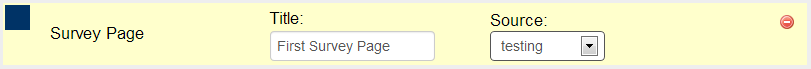
\includegraphics[width=5.0in]{figures/add_survey.png}
 \caption{Survey Page Inserted}
 \label{fig:surveyInsert}
\end{figure}
\FloatBarrier

\subsubsection {Asset Manager}

\begin{figure}[h!]
 \centering
 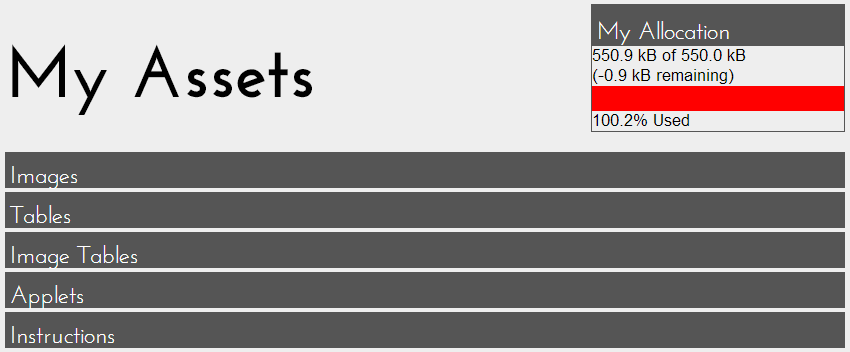
\includegraphics[width=5.0in]{figures/manage_assets.png}
 \caption{Asset Manager}
 \label{fig:manageAsset}
\end{figure}
\FloatBarrier

The asset manager allows you to upload images, table files, applets, and scripted components to your training pages.  Please note that applets and script components are grouped together.  The available assets for each type can be viewed from the dropdown menu underneath the corresponding category.  To manage a particular asset type, click on the section header for that type, and use the interface displayed.  The interface for each asset type is explained in greater detail below in the sections corresponding to each type.

Each administrator is allocated a certain amount of storage space to upload assets.  How much storage they get is dictated by the database, as explained in \textbf{Appendix A}.  When an administrator has reached their storage limits, they will be unable to load more assets until they remove other assets, or their capacity is increased by the system administrator.

\paragraph{Images}

\begin{figure}[h!]
 \centering
 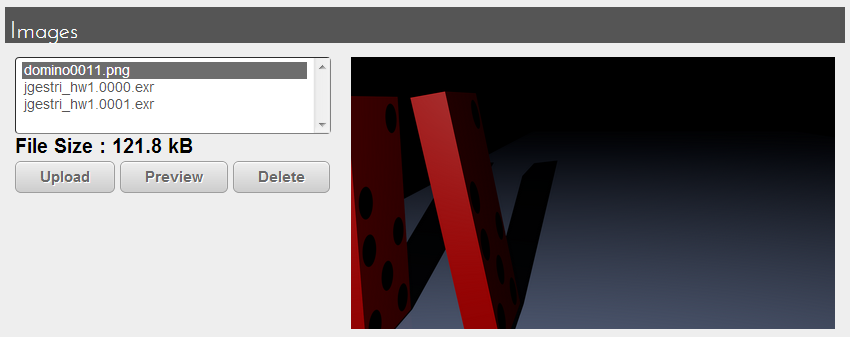
\includegraphics[width=5.0in]{figures/manage_images.png}
 \caption{Managing Image Assets}
 \label{fig:manageImg}
\end{figure}
\FloatBarrier

Figure \ref{fig:manageImg} shows the interface used to upload and manage image assets.  Images that are currently available on the system are listed in the text box on the left. To upload an imange, click on the button labeled \textbf{Upload} and select the file that you wish to upload. It is possible to preview these images by selecting the desired image and clicking on the button labeled, \textbf{Preview}.  The image will be displayed in the window on the right side of the interface.  To remove an asset from the list, select the asset and click on the button labeled \textbf{Delete}.

Dynasearch supports most major image formats.

\paragraph{Tables}

\begin{figure}[htb]
 \centering
 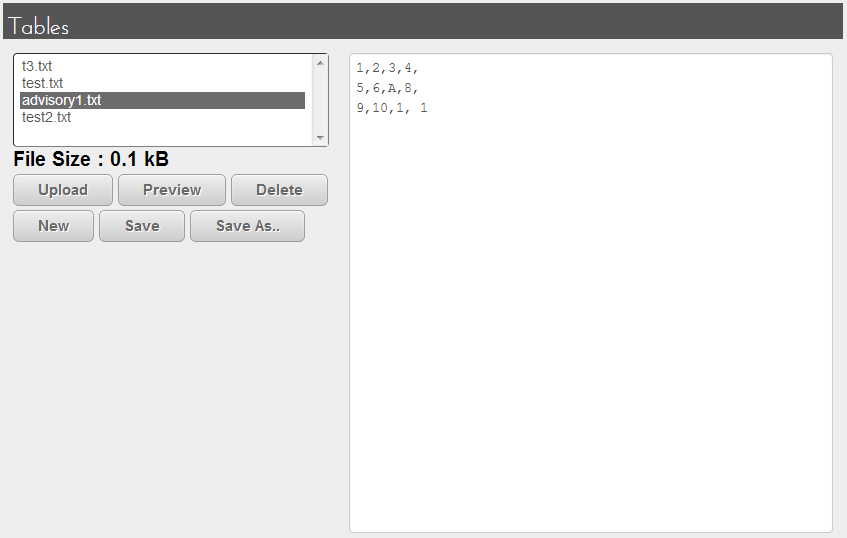
\includegraphics[width=5.0in]{figures/manage_tables.png}
 \caption{Managing Table Assets}
 \label{fig:manageTab}
\end{figure}
\FloatBarrier

The tables are just text files that are formatted so that columns are separated by commas and the rows are separated by new lines.  The interface to interact with table assets is show in Figure \ref{fig:manageTab}.  Tables  that are currently available on the system are listed in the text box on the left. To upload a prexisting table file, click the button labeled \textbf{Upload} and select the desired file.  To view the contents of a table file, click on the desired file from the list on the left and click on the button labeled \textbf{Preview}.  The file will be loaded in the text editor to the right in the interface.  To remove an asset from the list, select the asset and click on the button labeled \textbf{Delete}.

It is possible to edit and save table assets directly.  Clicking on the button labeled \textbf{New} will completely clear the text editor on the right.  Note that any changes given in the text editor will be lost when the \textbf{New} button is selected.  To save the contents of a file that have been edited, click on the button labeled \textbf{Save}.  To save the contents of the editor as a new table asset, click on the button marked \textbf{Save As} and enter the desired name to save the asset as.

\paragraph{Applets}

\begin{figure}[htb]
 \centering
 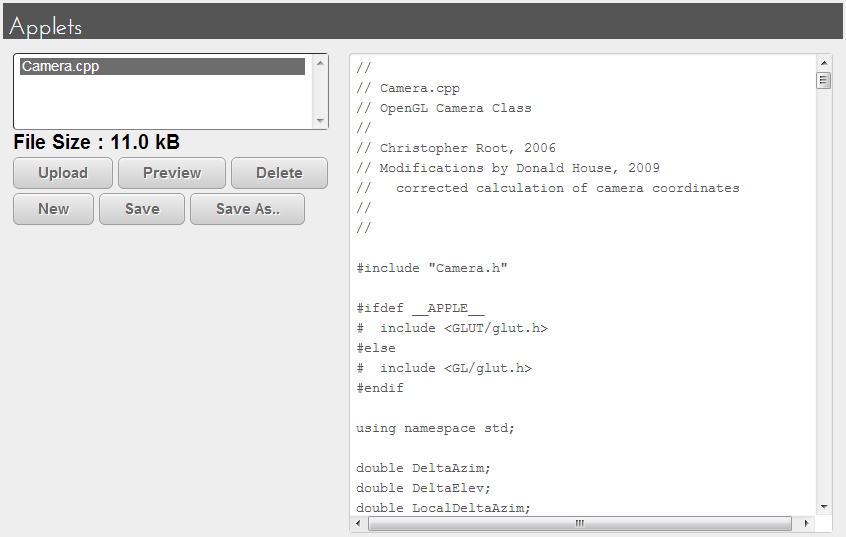
\includegraphics[width=5.0in]{figures/manage_applets.png}
 \caption{Managing Applet and Script Assets}
 \label{fig:manageApp}
\end{figure}
\FloatBarrier

Applets allow for a tremendous degree of flexibility when designing the training page at the cost of an additional development burden on the administrator.  With them, almost any kind of interaction can be built and incorperated into experiments through the training page.  Currently, applets can be Java Applets, or HTML 5 code that embeds WebGL, Processing, or D3.

The interface to interact with applet assets is show in Figure \ref{fig:manageApp}.  Applets and scripts that are currently available on the system are listed in the text box on the left. To upload a prexisting applet or script into the editor, click the button labeled \textbf{Upload} and select the desired file.  To view the contents of an asset file, click on the desired file from the list on the left and click on the button labeled \textbf{Preview}.  The file will be loaded in the text editor to the right in the interface.  To remove an asset from the list, select the asset and click on the button labeled \textbf{Delete}.

It is possible to edit and save applet and script assets directly.  Clicking on the button labeled \textbf{New} will completely clear the text editor on the right.  Note that any changes given in the text editor will be lost when the \textbf{New} button is selected.  To save the contents of a file that have been edited, click on the button labeled \textbf{Save}.  To save the contents of the editor as a new applet or script asset, click on the button marked \textbf{Save As} and enter the desired name to save the asset as.

\paragraph{Instructions}

\begin{figure}[htb]
 \centering
 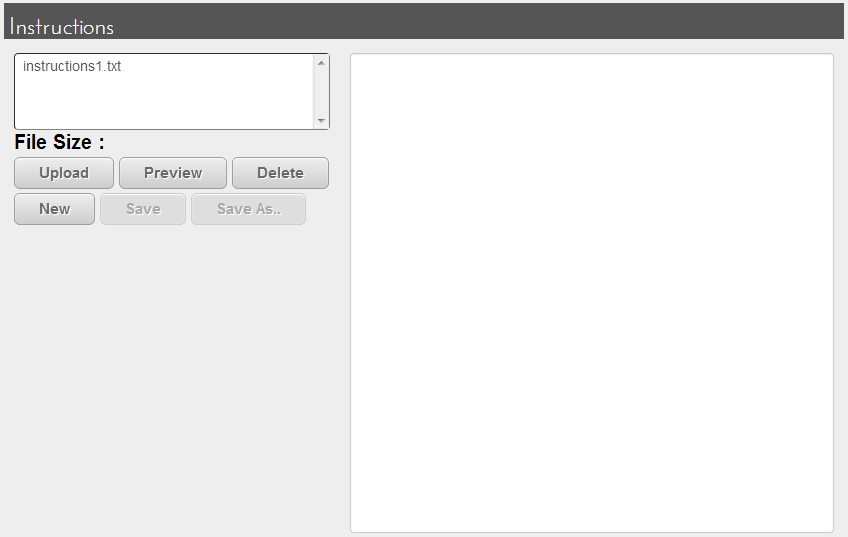
\includegraphics[width=5.0in]{figures/manage_instructions.png}
 \caption{Managing Instruction Assets}
 \label{fig:manageInst}
\end{figure}
\FloatBarrier

Instruction assets are text files that  display information to the users during the course of an experiment.  These files are loaded directly between the $<\texttt{body}>$ tags of an instruction page and can employ HTML 5 as well as scripting.

The interface to interact with instruction assets is show in Figure \ref{fig:manageInst}.  Instructions that are currently available on the system are listed in the text box on the left. To upload a prexisting instruction file, click the button labeled \textbf{Upload} and select the desired file.  To view the contents of an instruction file, click on the desired file from the list on the left and click on the button labeled \textbf{Preview}.  The file will be loaded in the text editor to the right in the interface.  To remove an instruction asset from the list, select the asset and click on the button labeled \textbf{Delete}.

It is possible to edit and save instructions assets directly.  Clicking on the button labeled \textbf{New} will completely clear the text editor on the right.  Note that any changes given in the text editor will be lost when the \textbf{New} button is selected.  To save the contents of a file that have been edited, click on the button labeled \textbf{Save}.  To save the contents of the editor as a new instruction asset, click on the button marked \textbf{Save As} and enter the desired name to save the asset as.

\subsubsection {Manage Participants}

\begin{figure}[h!]
 \centering
 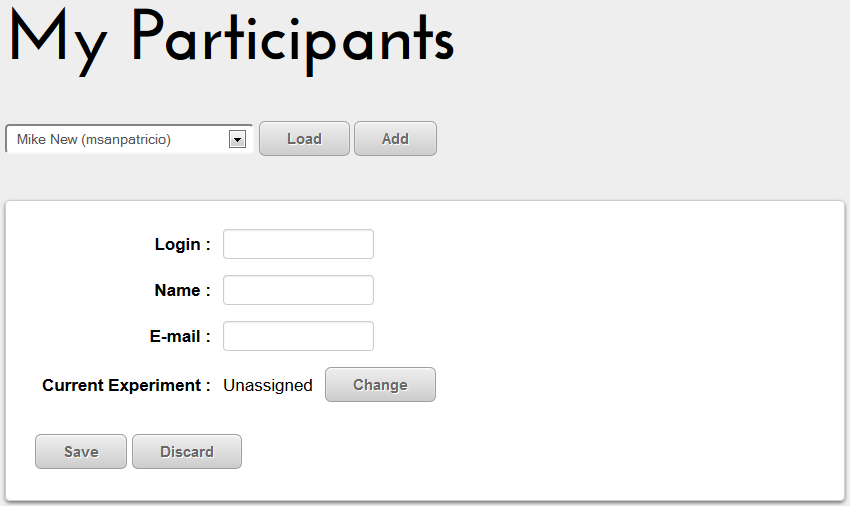
\includegraphics[width=5.0in]{figures/manage_participants_new.png}
 \caption{Participant Manager}
 \label{fig:managePartNew}
\end{figure}
\FloatBarrier

The participant manager allows administrators the ability to create and modify users.  To create a new user, click on the button labaled \textbf{Add}.  A form with the required fields for user creation is displayed, as is shown in Figure \ref{fig:managePartNew}.  All of these fields must be completed to create the user.

The \textem{Login} field is the name the user will login to DynaSearch with.  The \textem{Name} field is the user's name. The \textem{E-mail} field is user's email address.  After clicking on the button labeled \textbf{Save}, an email form will be displayed that will be used to notify the user of their account creation, as well as to provide them with a link to reset their password.

It is possible to assign users to an experiment upon user creation by clicking on the button labeled \textbf{Change} located next to the \textem{Current Experiment} field, but it is not required to create a user.

\begin{figure}[h!]
 \centering
 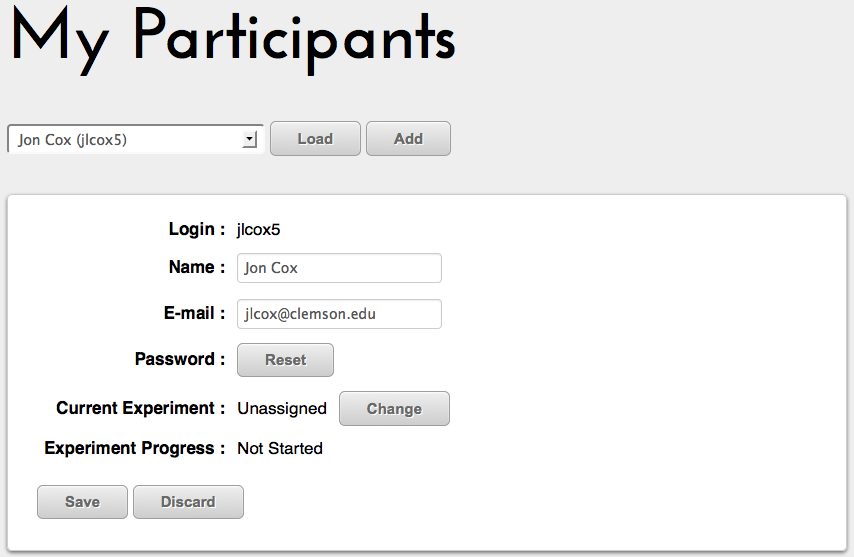
\includegraphics[width=5.0in]{figures/manage_participants.png}
 \caption{Participant Manager}
 \label{fig:managePart}
\end{figure}
\FloatBarrier

To modify an exisiting user select their name from the drop down list and click on the button labeled \textbf{Load}.  All of their information will be displayed, as show in Figure \ref{fig:managePart}.  Please note that administrators will only be able to change users that they have created.  This is important when mulitple administrators use the same system.

To assign a user to a specific experiment, click on the button labeled \textbf{Change} located next to their currently listed experiement, and select the desired experiement from the popup that is displayed.  Please note that the progress on the experiment the user is currently working on will be lost. The user's current progress in the designated experiment is shown next to the label \textbf{Experiment Progress}. 

In order to reset a user's password, the button labeled \textbf{Reset} must be selected.  This sends an email to the user with a link that will allow them to reset their password through the DynaSearch site.  This link will be valid for a predetermined period of time, after which point it will expire.

To save any changes made to a user account, click on the button labeled \textbf{Save}


\subsubsection {Results Manager}

\begin{figure}[h!]
 \centering
 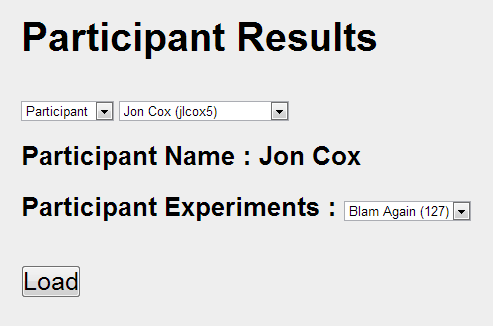
\includegraphics[width=5.0in]{figures/part_results.png}
 \caption{Results Manager}
 \label{fig:partResults}
\end{figure}
\FloatBarrier

The results for each study can be viewed and downloaded from the \testbf{Results Manger}, as shown in Figure \ref{fig:partResults}.  To do this, select the desired user from the dropdown list and then hit the button labaled \testbf{Load}.  Then, select the experiment you wish to review the results of and again hit the button labeled \textbf{Load}.

This will show a set of tables that display both the questionnaire data as well as the click data.  To download this, choose whether to download the click data or the questionnaire results, select the format desired (currently only plain text is supported), and hit the button labeled \textbf{Download}.  The details of the formats are specified below.

\paragraph{Plain Text}


\section{Administrator Settings}

\begin{figure}[h!]
 \centering
 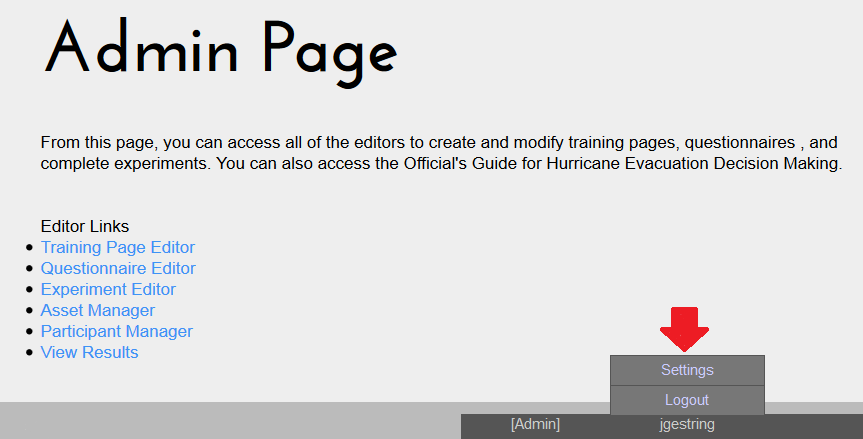
\includegraphics[width=5.0in]{figures/findSettings.png}
 \caption{Navigating to the Administrator Settings}
 \label{fig:findSettings}
\end{figure}
\FloatBarrier

The Administrator Settings screen is available to administrators by hovering over their name on the bottom pannel of the screen, and then selecting the link called \textem{Settings} from the menu that is displayed, as showin in Figure \ref{fig:findSettings}.

\subsection{Change Password}

\begin{figure}[h!]
 \centering
 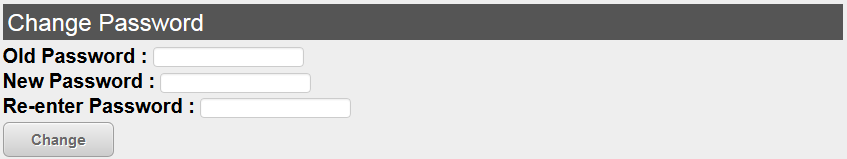
\includegraphics[width=5.0in]{figures/adminPassword.png}
 \caption{Changing an Administrator's Password}
 \label{fig:adminPassword}
\end{figure}
\FloatBarrier

To change your password, enter your current password in the field labeled \textem{Old Password}, and type and then retype your password in the fields marked \textem{New Password} and \textem{Re-enter Password} respectively as shown in \ref{fig:adminPassword}.  That's right.  Just like 90\% of all other password reset mechanisms in existence. 

\subsection{Change Email Address}

\begin{figure}[h!]
 \centering
 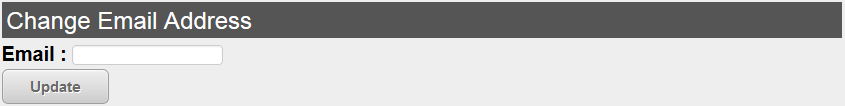
\includegraphics[width=5.0in]{figures/adminEmail.png}
 \caption{Changing an Administrator's Email Address}
 \label{fig:adminEmail}
\end{figure}
\FloatBarrier

\subsection{Screen Size Profile}

\begin{figure}[h!]
 \centering
 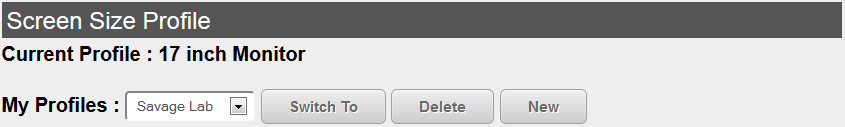
\includegraphics[width=5.0in]{figures/adminScreenProf.png}
 \caption{Setting and Changing Screen Profiles}
 \label{fig:adminScreenProf}
\end{figure}
\FloatBarrier

\section{Appendix A: Database Information}
The tables listed below are used for the DynaSearch system. Any other tables you find in the database are legacy items from the original EMDSS application on which this website was based. The tables have no dependency on each other. Because of this, the resulting structure is very simple and easy to maintain. The tables are explained in greater detail below. The database used for DynaSearch is MySQL 5.1. The entire system was built using version 2.0 of wampServer.


\subsection{sur\_question}
This table holds all of the questionnaires that have been created within DynaSearch. Everything in this database is handled internally, so it should almost never need to be accessed. It should be noted that once experiments are created, the information in the Value field is copied to a file in the file system. This is designed to protect individual experiments from issues that may occur with the database. The details of each field are given below.

\subparagraph{id}
The id field serves as the primary key for an entry. It should never need to be referenced.

\subparagraph{Admin\_ID}
This is the user name of the administrator that created the question.  Administrator's will only have access to the questions that they have created.

\subparagraph{Name}
This is the name of the given questionnaire. It is what is displayed when trying to insert the questionnaire into different experiments. Each should be unique.

\subparagraph{Value}
This is the HTML that makes up the questionnaire. It is stored in its basic format. If the questionnaire needs to be edited in any way after it is saved, it will have to be through this field, as there is currently no way to modify pre-existing surveys. 


\subsection{t\_experiments }
The experiments table holds all of the information that is saved from the Experiment Editor. Short of removing experiments from the database, this table should rarely be referenced. 

\subparagraph{id} 
The id field serves as the primary key for an entry. It should never need to be referenced. 

\subparagraph{ExperimentShortName}
The experiment short name is the name of the experiment that will be seen from the Experiment Editor. It will be the name given to the experiment on creation without any spaces or special characters.

\subparagraph{Admin\_ID}
This is the user name of the administrator that created the experiment.  Administrator's will only have access to the experiments that they have created.

\subparagraph{ScaleProfileID}
The ScaleProfileID field is used to determine which scale profile should be used for an experiment.  These scale profiles are stored in the database table \texttt{t\_scale\_profiles}.

\subparagraph{ExperimentString}
This field contains a string which represent the experiment referenced. Most of it is stored in hexadecimal characters, and is therefore unreadable by itself. This informa.tion should only ever be accessed through the Experiment Editor. This string keeps track of the order of the pages, as well as the names of the files that correspond to each page in the experimentÕs folder. 


\subsection{m\_turk}
This table holds the information required for integration into Amazon's Mechanical Turk.

\subparagraph{MT\_ID}
The mechanical turk identification number.

\subparagraph{Admin\_ID}

\subparagraph{Amazon\_ID}


\subsection{t\_scale\_profiles}
This table holds all of the scale profiles that are used to resize experiments as they are being run.  Scale profiles are created and set by administartors from their \textbf{Settings} screen.

\subparagraph{Profile\_ID}
The identification number used to associate scale profiles to experiments.

\subparagraph{Admin\_ID}
This is the user name of the administrator that created the scale profile.  Administrator's will only have access to the scale profiles that they have created.

\subparagraph{Name}
This is the name shown to the administrator in their \textbf{Settings} screen when they select which scale profile to use.

\subparagraph{scaleW}
This field only applies to users. It is the width measurement that is recorded from the size registration page, and is used to ensure that every element on a training page is displayed with proper proportion, regardless of the monitorÕs screen size or resolution. 

\subparagraph{scaleH}
This field only applies to users. It is the height measurement that is recorded from the size registration page, and is used to ensure that every element on a training page is displayed with proper proportion, regardless of the monitorÕs screen size or resolution. 


\subsection{t\_user}
This table holds all of the account information for a given user. A detailed look at the fields is given below.

\subparagraph{User\_ID}
This is the identification that the user provides to the login screen in order to access the experiment.

\subparagraph{Admin\_ID}
This is the user name of the administrator that created the user.  Administrator's will only have access to the users that they have created.

\subparagraph{Email}
This is the email account associated with the user's account.  This is used for resetting the passwords of users through the \textbf{Participant Manager} screen.

\subparagraph{MemoryAllocation}
This represents how much storage space administrators have for uploading all of their assets.  This value is in MB.

\subparagraph{County\_ID}
Lists the current county of the user. This field is currently not used. 

\subparagraph{PasswordHash}
This is the password for the user account.  These values are hashed for security reasons, and there is no direct way to determine the value of the password from an administrative standpoint.  They only way to change a user's password is to use the reset functionality available from the \textbf{Participant Manager} screen.

\subparagraph{User\_Type}
This specifies the role of the account. An "A" designates the account as an adminis.trator. If this is true, they will automatically taken to the administrator page on login. A "U" designates the account as user, and an "M" designates a user as a Mechanical Turk user. On login these individuals will be taken to the experiment they are participating in. They should not have access to any of the editors or administrator page. 

\subparagraph{Name}
Real name of the user. 

\subparagraph{ScaleProfileID}
This gives the identification number of the scale profile that should be associated with a user when they log in to perform an experiment.

\subparagraph{current\_position}
This field only applies to users. It determines where in an experiment the user should be, should they log out and try to log back in before the completion of the experiment. It should also prevent users from trying to back track in an experiment, though this behavior may vary from browser to browser. 

\subparagraph{experiment}
This field only applies to users. It determines which experiment will be displayed for a user when they log into the system. The value must be one of the Experiment Short Name entries listed in the t experiments table. 

\subparagraph{Current\_Experiment\_ID}
This field only applies to users. It determines which experiment will be displayed for a user when they log into the system. The value must be one of the experiment ID entries listed in the \texttt{t\_experiments }table. 

\subparagraph{ResetToken}
The reset token is generated when an administrator resets a user's password through the \textbf{Participant Manager} screen.  The link in the email redirects the user to DynaSearch and passes the token, which allows the user to reset their password.

\subparagraph{TokenExpiration}
This indicates the expiration date of the assocaited \texttt{ResetToken}.

\section{Appendix B: Filesystem Information}
The file system is separated into five sections. These are the main files, experiment files, experiment resources, user data, and other assets. Each of these is detailed below.

\subsection{Main Files}
The main DynaSearch directory contains the files that are used during interaction with and creation of experiments. A quick overview is given of the most notable files.

\paragraph{admin.php} - The page that administrators login to

\paragraph{advance.php and director.php} - These files interact to ensure that users go to the right page when they login and click through the experiment

\paragraph{dynaview.php} - The main training page that users interact with

\paragraph{editor.php} - This is the page where the Training Page Editor loads

\paragraph{instructions.php} - This is the page that is used to display instructions to the users 

\paragraph{questDisplay.php} - This page is used to implement the Questionnaire Viewer

\paragraph{questEditor.php} - This page is used to implement the Questionnaire Editor 

\paragraph{question.php} - This page is used to display questionnaires to users 

\paragraph{randQuestEditor.php} - This page is used to implement the Questionnaire Catalog 

\paragraph{survey\_setup.php} - This page is used to implement the Experiment Editor

\subsection{Administrator Filesystem}
A folder is created for each administrator that is used for storage and organizational purposes.  These folders are located in the \texttt{DynaSearch/admins} directory.  The name of the each folder corresponds to the username of the administrator that owns it.  Currently, these directories are only used to store the assets uploaded by the administrators.

The base folder that contains all of the assets for each administrator is located in the \texttt{DynaSearch/admins/[admin\_username]/assets} directory, where [admin\_username] is the username of the administrator that owns the folder.  The folders found in this directory as well as their purpose are listed below.

\paragraph{applets}
This directory contains all of the applets that have been uploaded by the administrator.  These can range from Java applets, Processing or D3 files, or HTML 5 files that have embeded scripings, such as WebGL.

\paragraph{images}
This directory contains all of the image assets loaded by the administrators.  DynaSearch supports most major image formats.

\paragraph{tables}
This directory contains all of the files containing table information which can be used in the training pages.

\paragraph{image\_tables}
This directory contains all of the image table files which are used in the training pages for chaging the images an image window displays based on the grid cell in the table that is clicked.

\paragraph{instructions}
This directory holds all of the files used in the instruction pages.  They can be just straight text or can contain HTML 5 and scripting elements.

\paragraph{text}
This directory holds all of the files that are used in the text boxes on the training screens.  These files should only contain text, and should be clear of any code or scripts.

\paragraph{training}
No longer in use %Legacy?

\subsection{Other Assets}
The \texttt{DynaSearch/assets} directory hold all of the background scripts and files that are used to make the DynaSearch system work. Below is a list of the subdirectories and any major files that are located in each.

\paragraph{images}
This directory holds all of the images utilized by DynaSearch.

\paragraph{php}
This directory holds all of the php files that are used behind the scenes.

\subparagraph{config.php} -Holds the database information that is required to access and modify data 

\subparagraph{standard.php} -Holds the standard header information for every php file. This includes the <head> tags. 
	
\subparagraph{db util.php} -Provides the connection to the database specified in config.php

\paragraph{scripts}
This directory holds all of the javascript files that are used in DynaSearch. There are a few notables files. 

\subparagraph{editor.js} -This is a rather large file that stores all of the functions used by the Training Page Editor and also by dynaview.php.
 	
\subparagraph{timer.js} -This file contains the scripts that are used to cover all of the elements on a training page, as well as to keep track of the user click information before it is sent to the server.

\paragraph{style}
This directory just holds the style information for DynaSearch.

\section{Appendix C: Installing Dynasearch}
To Install the DynaSearch Software:

1. Copy the DynaSearch folder to the appropriate folder utilized by the web server. 

2. Go the the Þle DynaSearch/assets/php/config.php and provide the 
appropriate information for the following: 


\emph{DB HOST} -this is the host name where the database is located
	
\emph{DB USER} -this is the administrator account that will be able to log in, query, and make changes to the EMDSS database
	
\emph{DB PASS} -this is the password for DB USER account
	
\emph{Note} -Do not change the database name unless the name is also changed 
on the database server 

3. Import the EMDSS database into the MySQL server. The database Þle is named EMDSS DB.sql.zip and can be found in the DynaSearch directory. 


4. To test whether the system was imported correctly, go to *webaddress*/DynaSearch/login.php with the user name jlcox5 with the password jlcox5. It should take you to a test.ing page. 

If there are any problems or questions, please contact: 
Jonathan Cox at jlcox@g.clemson.edu 
%% The Acknowledgements part is started with the command \acknowledgements;
%% acknowledgements are then done as normal sections before appendix
%% \acknowledgements

\acknowledgements

This work was supported in part by NSF and NOAA under grant NSF CHI 2008001386.


%% The Appendices part is started with the command \appendix;
%% appendix sections are then done as normal sections and after Acknowledgements
%% \appendix

%% \section{}
%% \label{}

%% References without bibTeX database:

%\begin{thebibliography}{-8}

%% \bibitem must have the following form:

%\small{
%\bibitem{key}

%...

%}

%\end{thebibliography}

%% References with bibTeX database:

\bibliographystyle{IJ4UQ_Bibliography_Style}

\bibliography{hurricane}
\end{document}
